%%% Содержимое слайдов

% 1. Название, автор, руководитель.
% 2. Постановка задачи (актуальность)
% 3. способ (инструменты для) решения
% 4. результаты
% 5. анализ результатов
% 6. Заключение 

\frame[plain]{\titlepage} % Титульный слайд

%-------------------------------------------------------------------------------

\section{Тематика работ НИР}

\begin{frame}
\frametitle{\insertsection}

\textbf{Три направления работ:}
\begin{enumerate}
    \item Фильтрация в неоднородных средах
    \item Электрометрия -- теория БКЗ
    \item Распараллеливание программ -- практическая работа
\end{enumerate}
\end{frame}

%-------------------------------------------------------------------------------
%-------------------------------------------------------------------------------

\section{Фильтрация в неоднородных средах}

%-------------------------------------------------------------------------------

\subsection{Постановка задачи}

\begin{frame}
\frametitle{\insertsection}
\framesubtitle{\insertsubsection}

\textbf{Начально-краевая задача}:
\begin{alignat*}{6}
    \frac{\partial}{\partial t} ( m \rho_i s_i )
    + \frac{\partial}{\partial x} ( \rho_i w_i ) = 0, &
    \qquad & x &\in (0, l), \ && t \in (0, T],
    \\
    w_i = - k \frac{k_i}{\eta_i} \frac{\partial p}{\partial x}, \
    s_w + s_o = 1, &
    & i &\in [w, o]. &&
\end{alignat*}
\vspace{-0.5cm}
\begin{alignat*}{6}
    s &= s_0(t), \ & p &= p_0(t),
    & \qquad x &= 0, \ & t &\in (0, T],
    \\
    & & p &= p_l(t),
    & \qquad x &= l, & t &\in (0, T],
    \\
    s &= s^0(x), \ & p &= p^0(x),
    & \qquad x &\in [0, l], \ & t &= 0.
\end{alignat*}

\begin{minipage}[t]{0.47\linewidth}
\textbf{Модель 1} \\
$\rho_i = \mathrm{const}$
\end{minipage}
\hfill
\begin{minipage}[t]{0.47\linewidth}
\textbf{Модель 2} \\
$\rho_i = \rho^0_i \cdot \exp \left( \chi_i \left( p - p_0 \right) \right)$
\end{minipage}
\end{frame}

%-------------------------------------------------------------------------------

\subsection{Способ решения}

\begin{frame}
\frametitle{\insertsection}
\framesubtitle{\insertsubsection}

\begin{itemize}
    \item Язык программирования C для реализации численных схем
    \item Метод IMPES для решения системы дифференциальных уравнений в теории фильтрации
    \item Метод конечных разностей для аппроксимации дифференциального уравнения с помощью системы алгебраических уравнений
    \item Метод Ньютона для решения системы нелинейных алгебраических уравнений
    \item Метод прогонки для решения системы линейных алгебраических уравнений с тридиагональной матрицей
\end{itemize}
\end{frame}

%-------------------------------------------------------------------------------

\subsection{Результаты}

\begin{frame}
\frametitle{\insertsection}
\framesubtitle{\insertsubsection}

\textbf{Поля физических величин во времени у моделей:}

\hspace{-0.9cm}
\begin{minipage}[t]{0.5\linewidth}
    \center{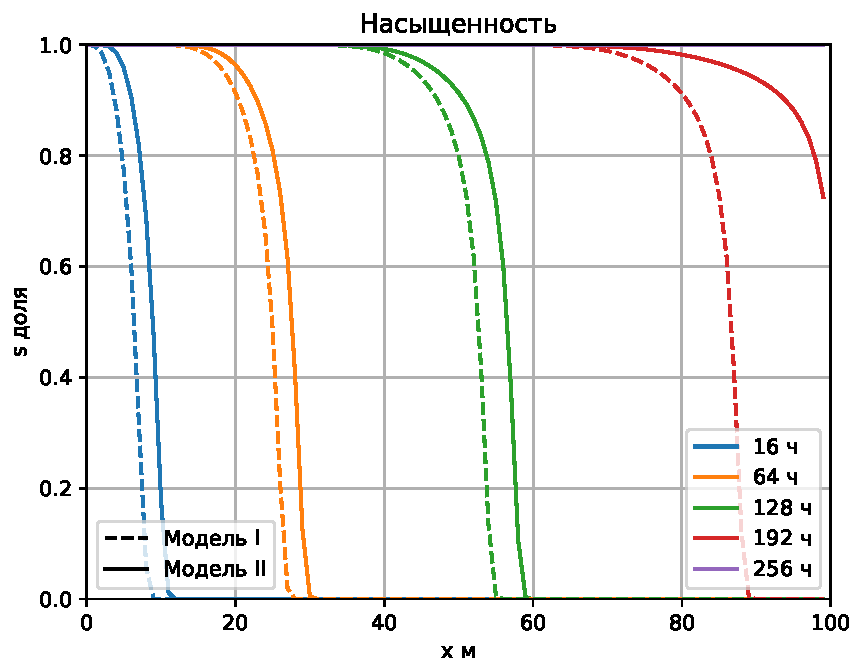
\includegraphics[height=0.9\linewidth]{filtration/palet_compare_mh_s_cropped.pdf}}
\end{minipage}
\hfill
\begin{minipage}[t]{0.5\linewidth}
    \center{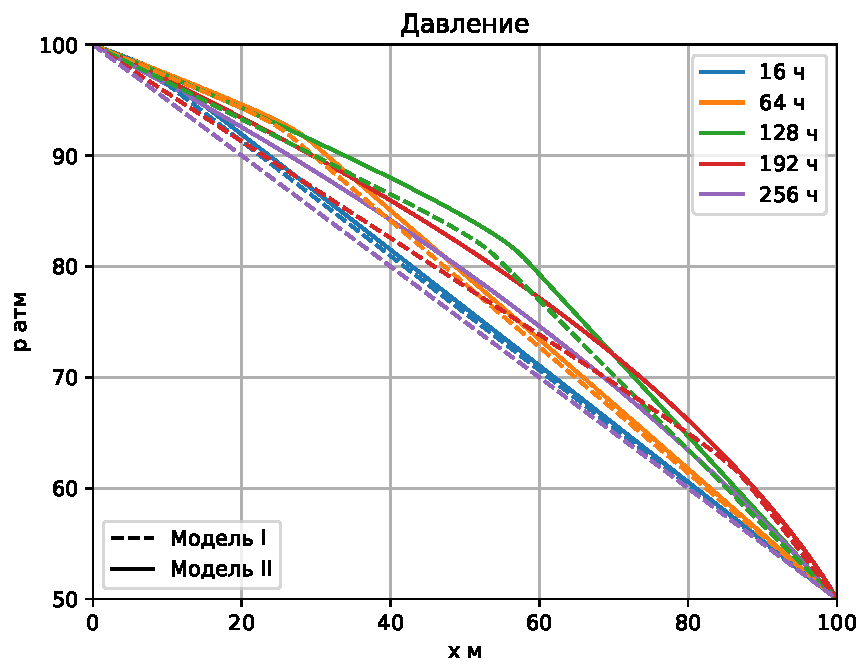
\includegraphics[height=0.9\linewidth]{filtration/palet_compare_mh_p_cropped.pdf}}
\end{minipage}
\end{frame}

%-------------------------------------------------------------------------------
%-------------------------------------------------------------------------------

\section{Электрометрия -- теория БКЗ}

%-------------------------------------------------------------------------------

\subsection{Постановка задачи}

\begin{frame}
\frametitle{\insertsection}
\framesubtitle{\insertsubsection}

\textbf{Краевая задача:}
\begin{alignat*}{2}
\nabla \cdot (\nabla u(\bm x) / \rho(\bm x)) &= -I \delta(\bm x),\qquad && \bm x \in \varOmega, \\
u(\bm x) &= 0, && \bm x \in \partial \varOmega.
\end{alignat*}

\begin{minipage}[t]{0.47\linewidth}
    \textbf{Модель 1}
    \center{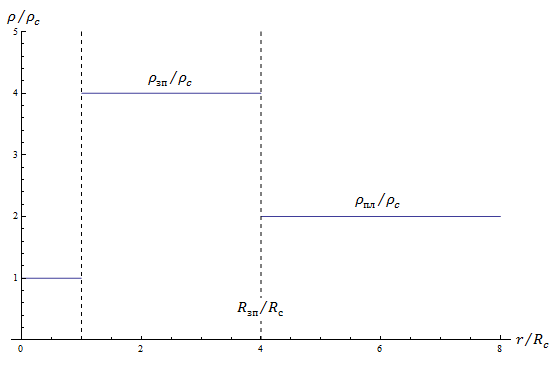
\includegraphics[width=1\linewidth]{electrometry/rho_model_1.png}}
\end{minipage}
\hfill
\begin{minipage}[t]{0.47\linewidth}
    \textbf{Модель 2}
    \center{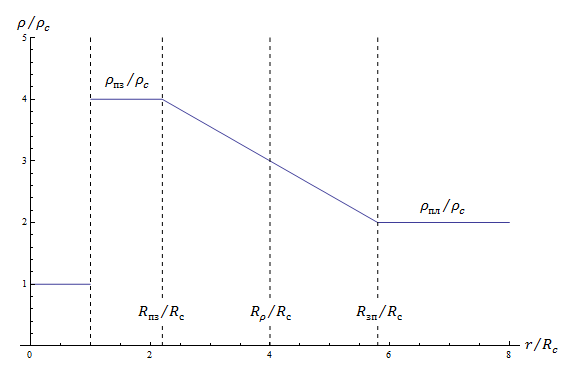
\includegraphics[width=1\linewidth]{electrometry/rho_model_2.png}}
\end{minipage}
\end{frame}

%-------------------------------------------------------------------------------

\subsection{Способ решения}

\begin{frame}
\frametitle{\insertsection}
\framesubtitle{\insertsubsection}

\textbf{Инструменты:}
\begin{itemize}
    \item Язык программирования Python
    \item Вычислительная платформа FEniCS -- метод конечных элементов
    \item Библиотека Numpy -- численные вычисления
    \item Библиотека triangle -- триангуляция расчетной области
    \item Компьютер: ОС Ubuntu 18.04 LTS, процессор Intel Pentium 4415U @ 2.30GHz
\end{itemize}
\end{frame}

% Построение расчетной сетки с заданием узлов и графа для триангуляции расчетной области с помощью библиотеки triangle.

% \begin{frame}
% \frametitle{\insertsection}
% \framesubtitle{\insertsubsection}
% 
% \textbf{Оптимальная расчетная схема:}
% \begin{itemize}
%     \item узлы на лучах
%     \item лагранжевы конечные элементы со второй степенью
%     \item отрезки графа на границах зон
%     \item узлы на пересечениях границ зон с лучами и окружностями
% \end{itemize}
% \bigskip
% 
% \textbf{Пример расчетной сетки модели 2}:
% 
% \begin{minipage}[t]{0.47\linewidth}
%     \center{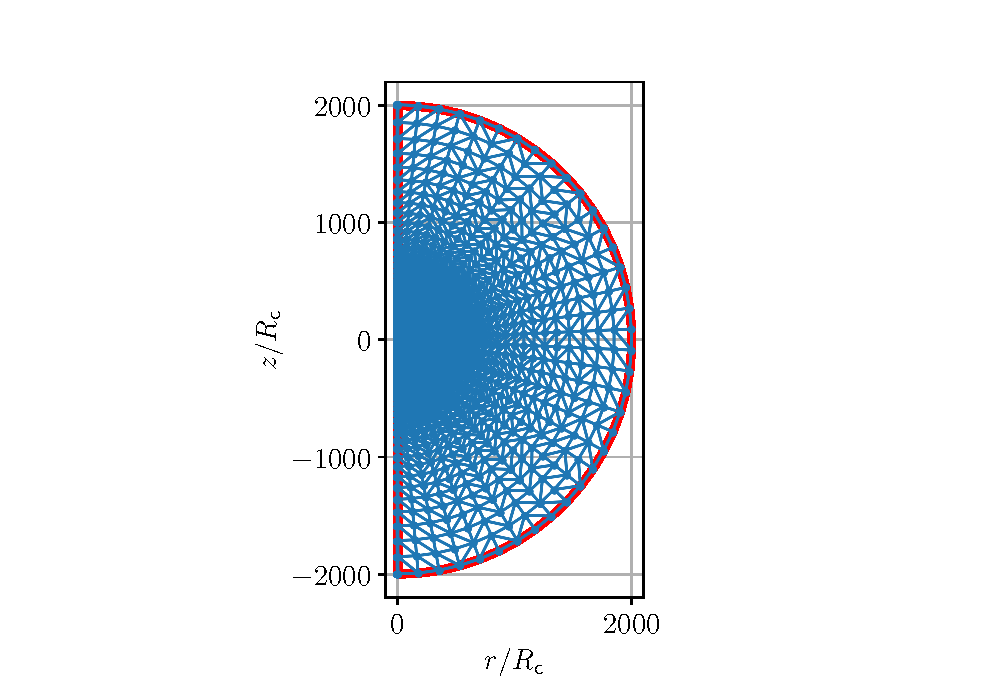
\includegraphics[width=1\linewidth]{electrometry/model_2_mesh_1_pres.pdf}}
% \end{minipage}
% \hfill
% \begin{minipage}[t]{0.47\linewidth}
%     \center{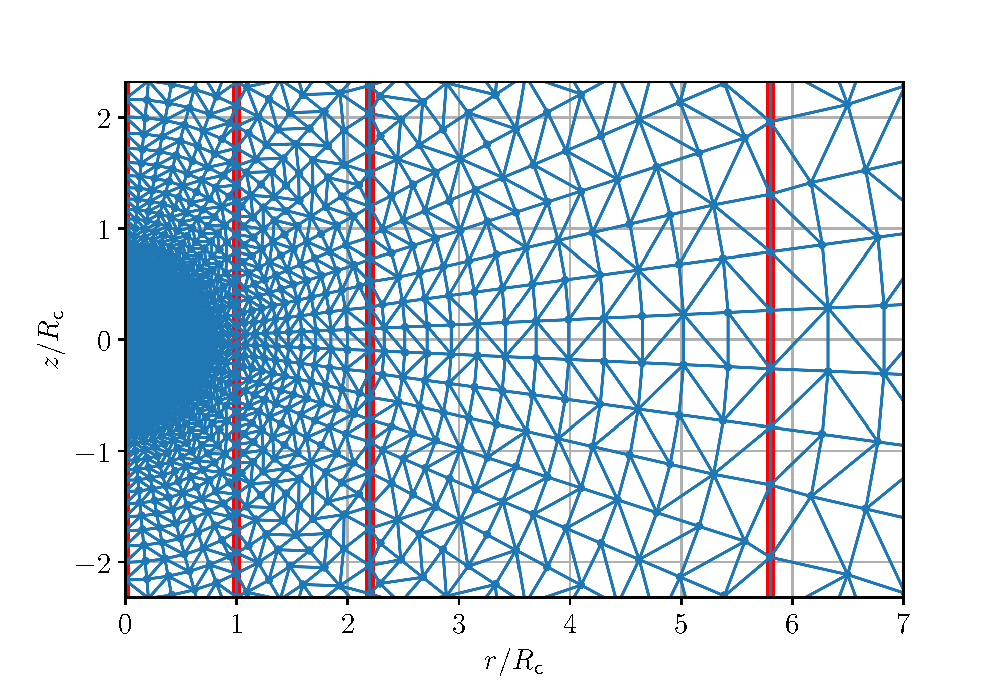
\includegraphics[width=1\linewidth]{electrometry/model_2_mesh_2_pres.pdf}}
% \end{minipage}
% \end{frame}

%-------------------------------------------------------------------------------

\subsection{Результаты}

\begin{frame}
\frametitle{\insertsection}
\framesubtitle{\insertsubsection}

\vspace{-0.5cm}
\begin{minipage}[t]{0.47\linewidth}
    \textbf{Модель 1}
    \center{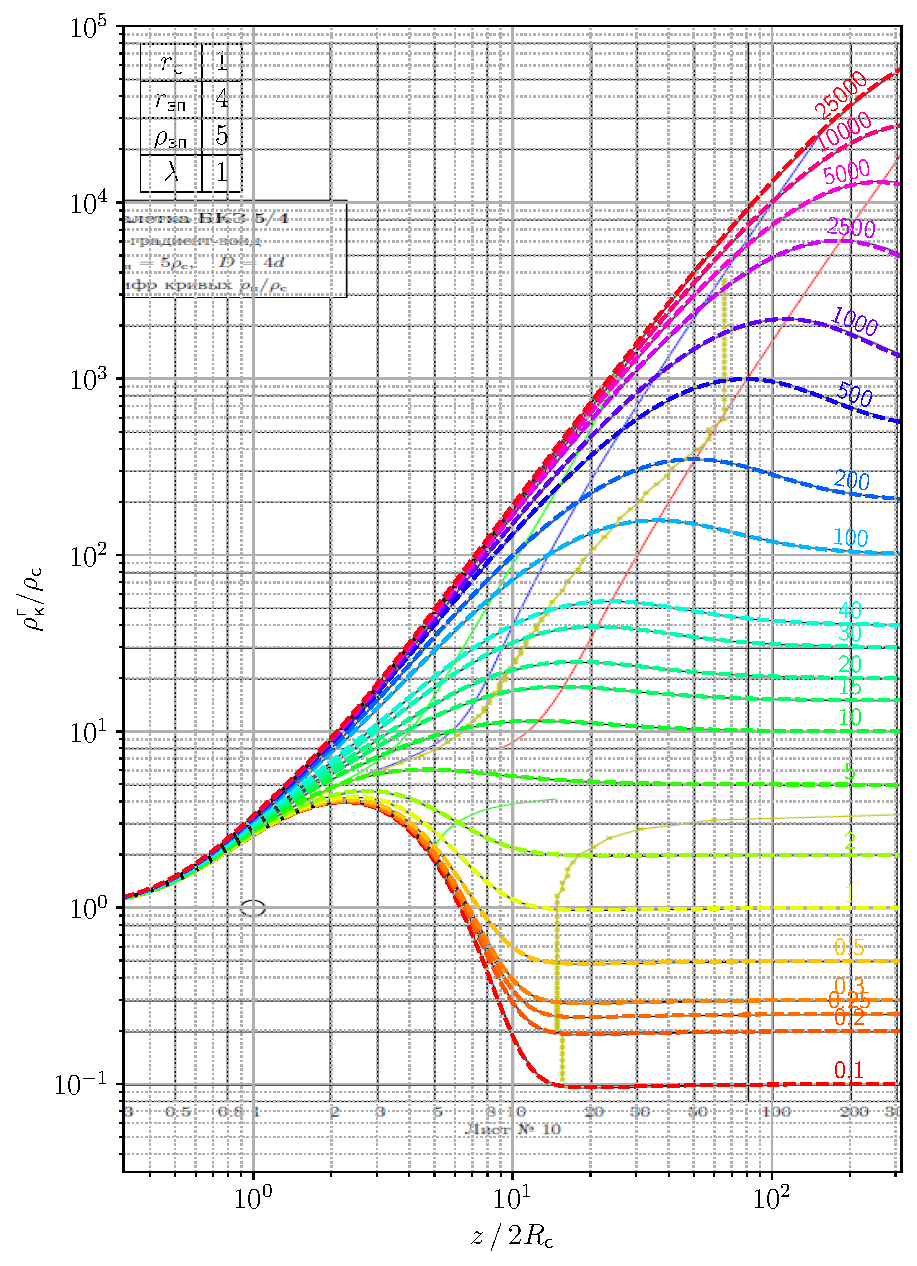
\includegraphics[width=1\linewidth]{electrometry/plot_1_compare}}
\end{minipage}
\hfill
\begin{minipage}[t]{0.47\linewidth}
    \textbf{Модель 2}
    \center{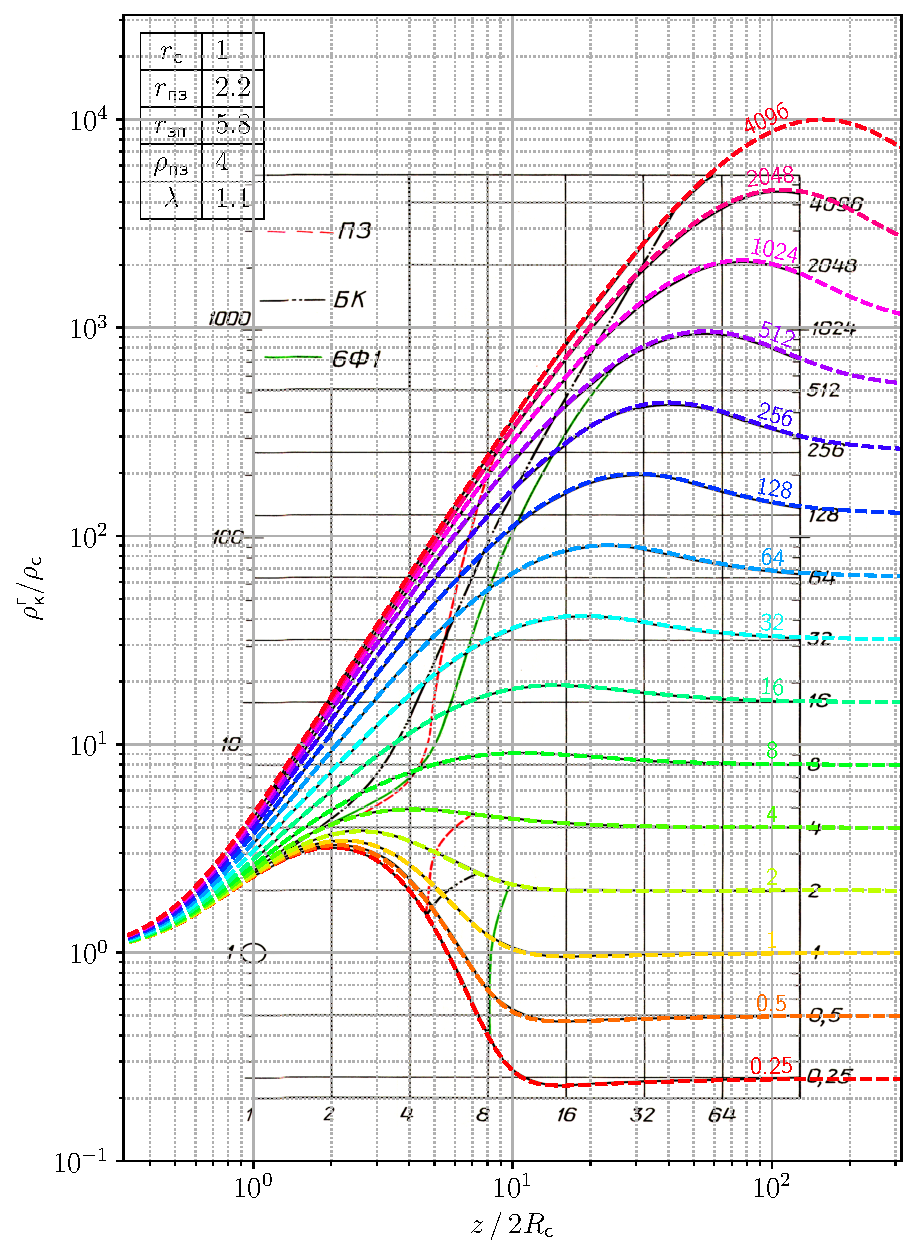
\includegraphics[width=1\linewidth]{electrometry/plot_2_compare}}
\end{minipage}

\end{frame}

%-------------------------------------------------------------------------------

% \subsection{Анализ результатов}
% 
% \begin{frame}
% \frametitle{\insertsection}
% \framesubtitle{\insertsubsection}
% 
% \textbf{Модель 1:}
% \begin{itemize}
%     \item Время вычисления расчетной палетки 15.981 с
%     \item 4669 узлов расчетной сетки
% \end{itemize}
% \bigskip
% 
% \textbf{Модель 2:}
% \begin{itemize}
%     \item Время вычисления расчетной палетки 11.905 с
%     \item 4813 узлов расчетной сетки
% \end{itemize}
% \bigskip
% 
% \textbf{Критерии точности решения}:
% \begin{itemize}
%     \item Гладкость решения
%     \item Сравнение "на глаз" решения с известным
% \end{itemize}
% \end{frame}

%-------------------------------------------------------------------------------
%-------------------------------------------------------------------------------

\section{Распаралелливание программ}

%-------------------------------------------------------------------------------

\subsection{Постановка задачи}
\begin{frame}
\frametitle{\insertsection}
\framesubtitle{\insertsubsection}

Эффективная утилизация ресурсов компьютера с помощью параллельного программирования
для решения задачи парсинга огромного текстового файла последовательности вещественных чисел,
не помещающегося в оперативную память, из носителя информации.

Парсинг -- автоматическое распознавание последовательности символов.
В нашем случае конкретно означает автоматический перевод текстовой записи вещественных чисел
в бинарную запись число с плавающей точкой.
\end{frame}

%-------------------------------------------------------------------------------

\subsection{Способ решения}


\begin{frame}
\frametitle{\insertsection}
\framesubtitle{\insertsubsection}

\textbf{Инструменты:}
\begin{itemize}
    \item Язык программирования С и стандартные библиотеки
    \item Расширение OpenMP языка C для распараллеливания программ 
    \item Компьютер: ОС Kubuntu 20.04 LTS, процессор  Intel i5-3330 @ 3.20GHz
\end{itemize}
\end{frame}

%-------------------------------------------------------------------------------
%-------------------------------------------------------------------------------

\section{Заключение}

\begin{frame}
\frametitle{\insertsection}
\framesubtitle{\insertsubsection}

\begin{itemize}
    \item Освоены пакеты программ для параллельных вычислений
    \item Разработаны прототипы программ
    \item Проведены расчеты и сопоставление
    \item Проведен анализ уравнений для различных моделей
    \item Получены численные реализации уравнений
    \item Показано применимость методов решения
\end{itemize}
\end{frame}

%-------------------------------------------------------------------------------

\section{Конец}

\begin{frame}[plain]
\centering
\btVFill
\textcolor{Blue}{\Large Спасибо за внимание!}
\btVFill
\end{frame}
